\documentclass[11pt,a4paper,titlepage]{report}


\usepackage[italian]{babel} %italiano
\usepackage[T1]{fontenc} 
\usepackage[utf8]{inputenc}
\usepackage{graphicx} %immagini
\usepackage{hyperref}
\usepackage{fancyhdr}
\usepackage[nouppercase]{frontespizio}
\usepackage{wrapfig} 
\usepackage{listings}

%-----------For json--------------
\usepackage{xcolor}
\colorlet{punct}{red!60!black}
\definecolor{background}{HTML}{EEEEEE}
\definecolor{delim}{RGB}{20,105,176}
\colorlet{numb}{magenta!60!black}
\lstdefinelanguage{json}{
    basicstyle=\normalfont\ttfamily,
    numbers=left,
    numberstyle=\scriptsize,
    stepnumber=1,
    numbersep=8pt,
    showstringspaces=false,
    breaklines=true,
    frame=lines,
    backgroundcolor=\color{background},
    literate=
     *{0}{{{\color{numb}0}}}{1}
      {1}{{{\color{numb}1}}}{1}
      {2}{{{\color{numb}2}}}{1}
      {3}{{{\color{numb}3}}}{1}
      {4}{{{\color{numb}4}}}{1}
      {5}{{{\color{numb}5}}}{1}
      {6}{{{\color{numb}6}}}{1}
      {7}{{{\color{numb}7}}}{1}
      {8}{{{\color{numb}8}}}{1}
      {9}{{{\color{numb}9}}}{1}
      {:}{{{\color{punct}{:}}}}{1}
      {,}{{{\color{punct}{,}}}}{1}
      {\{}{{{\color{delim}{\{}}}}{1}
      {\}}{{{\color{delim}{\}}}}}{1}
      {[}{{{\color{delim}{[}}}}{1}
      {]}{{{\color{delim}{]}}}}{1},
}
%---------------------------------------
%------------JavaScript-----------------
\lstdefinelanguage{JavaScript}{
keywords={typeof, new, true, false, catch, function, return, null, catch, switch, var, if, in, while, do, else, case, break},
keywordstyle=\color{blue}\bfseries,
ndkeywords={class, export, boolean, throw, implements, import, this},
ndkeywordstyle=\color{darkgray}\bfseries,
identifierstyle=\color{black},
sensitive=false,
comment=[l]{//},
morecomment=[s]{/*}{*/},
commentstyle=\color{purple}\ttfamily,
stringstyle=\color{red}\ttfamily,
morestring=[b]',
morestring=[b]"
}
%-------------------------------------------
\pagestyle{fancy}
\renewcommand{\chaptermark}[1]{\markboth{#1}{#1}}
\fancyhf{}
\fancyhead[R]{\small\bfseries\thepage}
\fancyhead[L]{\small\bfseries\thechapter\ \leftmark}
\setlength{\headheight}{13.6pt} 
\fancypagestyle{plain}{%
  \fancyhead{}\fancyfoot[C]{\thepage}%
  \renewcommand{\headrulewidth}{0pt}%
}

\graphicspath{ {./img/} }
\linespread{1.23}

% Copyright 2017 Sergei Tikhomirov, MIT License
% https://github.com/s-tikhomirov/solidity-latex-highlighting/

\usepackage{listings, xcolor}

\definecolor{verylightgray}{rgb}{.97,.97,.97}

\lstdefinelanguage{Solidity}{
	keywords=[1]{anonymous, assembly, assert, balance, break, call, callcode, case, catch, class, constant, continue, constructor, contract, debugger, default, delegatecall, delete, do, else, emit, event, experimental, export, external, false, finally, for, function, gas, if, implements, import, in, indexed, instanceof, interface, internal, is, length, library, log0, log1, log2, log3, log4, memory, modifier, new, payable, pragma, private, protected, public, pure, push, require, return, returns, revert, selfdestruct, send, solidity, storage, struct, suicide, super, switch, then, this, throw, transfer, true, try, typeof, using, value, view, while, with, addmod, ecrecover, keccak256, mulmod, ripemd160, sha256, sha3}, % generic keywords including crypto operations
	keywordstyle=[1]\color{blue}\bfseries,
	keywords=[2]{address, bool, byte, bytes, bytes1, bytes2, bytes3, bytes4, bytes5, bytes6, bytes7, bytes8, bytes9, bytes10, bytes11, bytes12, bytes13, bytes14, bytes15, bytes16, bytes17, bytes18, bytes19, bytes20, bytes21, bytes22, bytes23, bytes24, bytes25, bytes26, bytes27, bytes28, bytes29, bytes30, bytes31, bytes32, enum, int, int8, int16, int24, int32, int40, int48, int56, int64, int72, int80, int88, int96, int104, int112, int120, int128, int136, int144, int152, int160, int168, int176, int184, int192, int200, int208, int216, int224, int232, int240, int248, int256, mapping, string, uint, uint8, uint16, uint24, uint32, uint40, uint48, uint56, uint64, uint72, uint80, uint88, uint96, uint104, uint112, uint120, uint128, uint136, uint144, uint152, uint160, uint168, uint176, uint184, uint192, uint200, uint208, uint216, uint224, uint232, uint240, uint248, uint256, var, void, ether, finney, szabo, wei, days, hours, minutes, seconds, weeks, years},	% types; money and time units
	keywordstyle=[2]\color{teal}\bfseries,
	keywords=[3]{block, blockhash, coinbase, difficulty, gaslimit, number, timestamp, msg, data, gas, sender, sig, value, now, tx, gasprice, origin},	% environment variables
	keywordstyle=[3]\color{violet}\bfseries,
	identifierstyle=\color{black},
	sensitive=false,
	comment=[l]{//},
	morecomment=[s]{/*}{*/},
	commentstyle=\color{gray}\ttfamily,
	stringstyle=\color{red}\ttfamily,
	morestring=[b]',
	morestring=[b]"
}

\lstset{
	language=Solidity,
	backgroundcolor=\color{verylightgray},
	extendedchars=true,
	basicstyle=\footnotesize\ttfamily,
	showstringspaces=false,
	showspaces=false,
	numbers=left,
	numberstyle=\footnotesize,
	numbersep=9pt,
	tabsize=2,
	breaklines=true,
	showtabs=false,
	captionpos=b
}
 %solidity color
%\begin{lstlisting}[language=Solidity]
%\end{lstlisting}

\begin{document}

\begin{frontespizio}
\Universita{Torino}
\Facolta{Scieze della Natura}
\Corso[Laurea]{Informatica}
\Logo[7.5cm]{./img/Unito-logo}
\Titoletto{Tesi di laurea}
\Titolo{Studio e realizzazione di un prototipo di un sistema basato su blockchain per il mobility as a service}
\Candidato[880847]{Giorgio Mecca}
\Relatore{Prof.~Claudio Schifanella}
\Annoaccademico{2020-2021}
\end{frontespizio}

%\author{Giorgio Mecca}
%\title{Studio e realizzazione di un prototipo di un sistema basato su blockchain per il mobility as a service}
%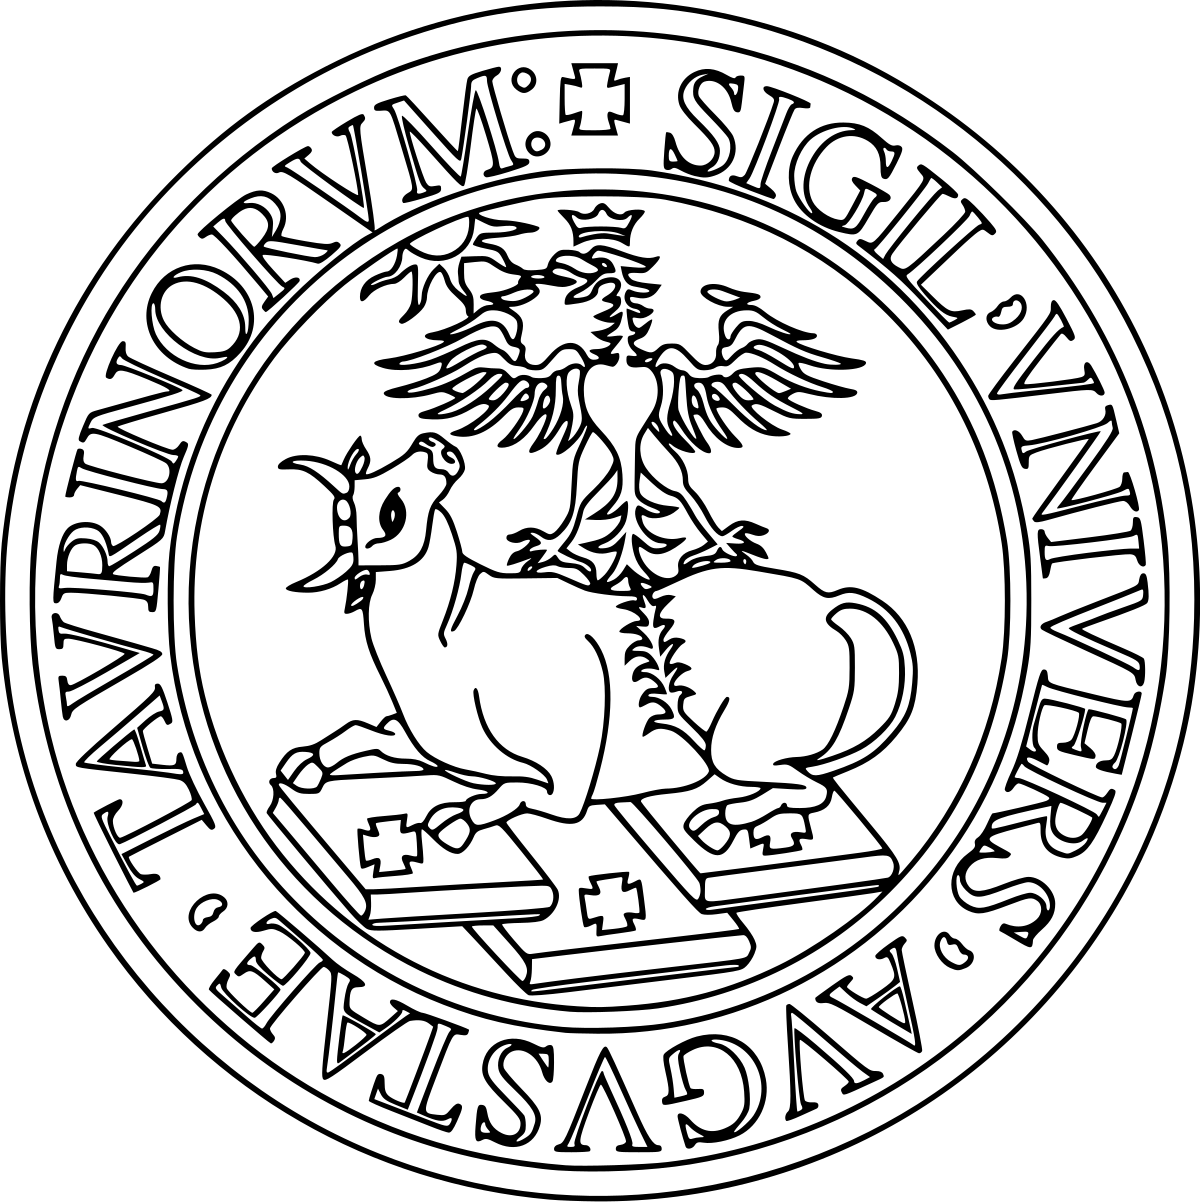
\includegraphics[height=.2\textheight]{Unito-logo}
%\maketitle
%Study and realization of a prototype of a blockchain-based system for mobility as a service

%indice
\tableofcontents

%capitolo 1
\chapter{Introduzione}
\section{Descrizione del Progetto}
\section{Descrizione dell’azienda}

%capitolo 2
\chapter{Blockchain}
\section{Problema dei generali bizantini}
\begin{figure}[h]
	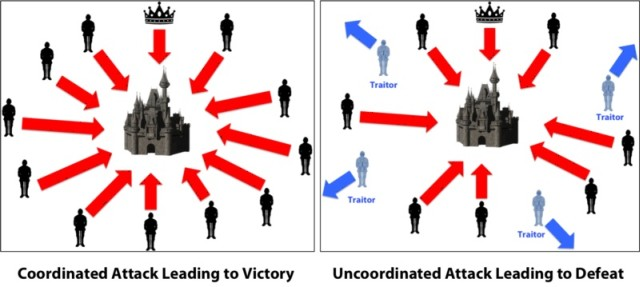
\includegraphics[width=\textwidth]{BF}
	\centering
	\caption{Problema dei generali bizantini}
	\label{fig:ByzantinFault}
\end{figure}

Il problema dei generali bizantini è un problema informatico su come raggiungere il consenso in situazioni in cui è possibile la presenza di errori. Il problema consiste nel trovare un accordo, comunicando solo tramite messaggi, tra componenti diversi nel caso in cui siano presenti informazioni discordanti. Il problema è stato teorizzato dai matematici Leslie Lamport, Marshall Pease e Robert Shostak nel 1982, i quali crearono la metafora dei generali, caso di studio molto utilizzato nei sistemi basati o che comunque utilizzano una network. La metafora si basa su diversi generali che durante un assedio sono sul punto di attaccare una città nemica. Essi sono dislocati in diverse aree strategiche e possono comunicare solo mediante messaggeri al fine di coordinare l'attacco decisivo (Figura \ref{fig:ByzantinFault}). I generali possono attaccare o ritirarsi, l'importante e che ci sia una decisione unanime, l'utilizzo di sola metà forza bellica porterebbe ad una sconfitta o una perdita. Il problema risiede quindi nell'alta probabilità che tra questi vi sia un generale traditore che mandi messaggi che vanno contro la strategia dell'esercito. La possibile soluzione punta al trovare un meccanismo secondo il quale un generale non traditore che riceva più messaggi sappia riconoscere quello veritiero. Secondo l'articolo di Lamport, Shostak e Pease non esiste una soluzione se il numero di processi non corretti è maggiore o uguale a un terzo del numero totale di processi. Una soluzione proposta è quella di Nakamoto che in una sua stesura sulla blockchain descrive un meccanisco per arrivare al consenso chiamato PoW Proof of Work.

\section{Struttura di una blockchain}
\begin{figure}[h]
	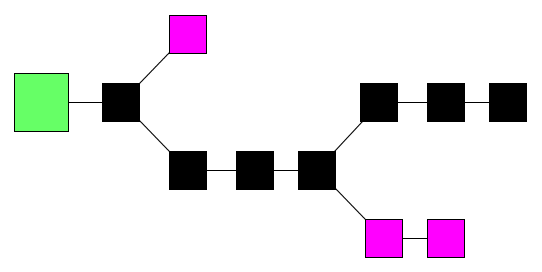
\includegraphics[width=\textwidth]{bl1}
	\centering
	\caption{Rappresentazione struttura di una blockchain}
	\label{fig:blockchain1}
\end{figure}

Una Blockchain come suggerisce l'etimologia della parola è una catena di blocchi o DLT - Distributed Ledger Technology. È una struttura dati formata da un insieme di blocchi(struttura prioritaria) collegati univocamente 1 ad 1 così da creare una metaforica catena. Una blockchain è considerata una struttura condivisa e immutabile in quanto il suo contenuto una volta scritto non è più né modificabile né eliminabile, a meno di non invalidare l'intera struttura. Questa tecnologia fà parte dei Distributed Legder cioè dei "libri mastro distribuiti" o registri condivisi, infatti tutti i partecipanti della blockchain, detti anche nodi, posseggono lo stesso registro. Essi posseggono le stesse informazioni costruendo il contrapposto di una struttura centralizzata come un Database, quindi una struttura Decentralizzata in cui ogni nodo ha la possibilità di leggere autonomamente le informazioni contenute.
Nella figura \ref{fig:blockchain1} viene visualizzata una semplice blockchain in cui sono presenti tre tipologie di blocchi quali: il blocco verde visto come il blocco di genes; i blocchi neri che vanno a costituire la catena principale e i blocchi viola considerati blocchi orfani. L'aggiunta di un nuovo blocco è globalmente regolata da un protocollo condiviso, se autorizzata ogni nodo aggiorna la propria copia privata del registro così da evitare manipolazioni future. In una blockchain i nodi partecipanti vengono anche chiamati minatori - miner o validatori, riferendosi al loro compito nella rete rispetto ai blocchi.

\section{Hashing}
Un codice hash è una qualunque sequenza di caratteri alfanumerici generati da una particolare funzione di hash. Questa funzione prende in input un qualunque tipo di informazione e restituisce una stringa di lunghezza prefissata, questo rende la funzione one-way o non invertibile in quanto conoscendo il digest(codice hash restituito) non è possibile risalire all'informazione che lo ha generato. In una blockchain l'Hash viene utilizzato per la costruzione della catena, viene calcolato l'hash di un blocco e il blocco successivo avrà come parametro questo hash. In questo modo ogni blocco è legato univocamente al blocco precedente "parent", siccome il codice hash di un blocco viene calcolato utilizzando anche il codice hash precedente modificando un singolo blocco verrà invalidata tutta la struttura blockchain immediatamente successiva.
\begin{figure}[h]
	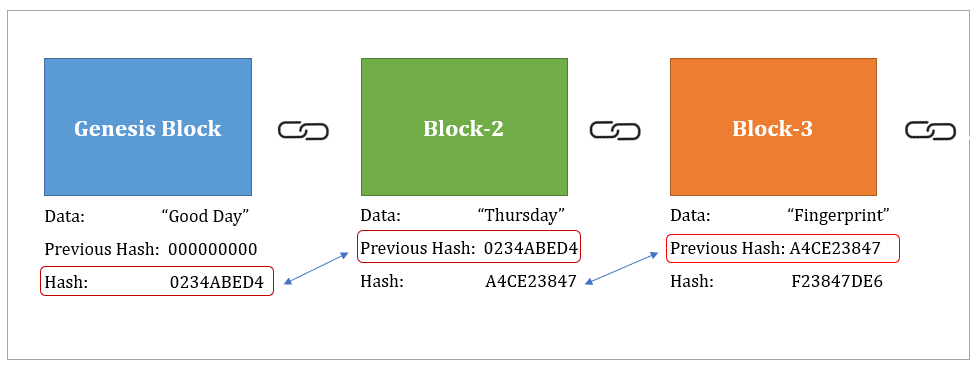
\includegraphics[width=\textwidth]{bc1}
	\centering
	\caption{Catena di una blockchain}
	\label{fig:blockchain2}
\end{figure}

\section{Transazioni}
\begin{figure}[h]
	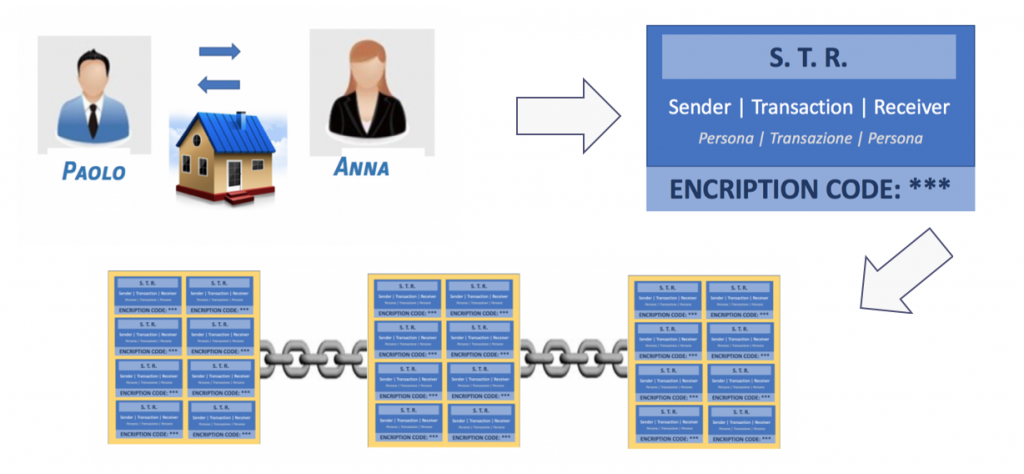
\includegraphics[width=\textwidth]{flusso_bc}
	\centering
	\caption{Flusso di esecuzione di una Transazione}
	\label{fig:fl_bc}
\end{figure}
In una blockchain i dati vengono scritti sotto forma di transazioni, in seguito contenute in vari blocchi. L'uso più comune delle transazioni è l'invio di denaro o una qualche tipologia di moneta equivalente. Le transazioni devono quindi avere un mittente, un destinatario, un 'value' cioè il valore trasmesso; vengono quindi considerate come un cambio di stato riferendosi alle informazioni nella blockchain e saranno identificate da un Transaction Hash. Una volta inviata, la transazione entra in una transaction pool, da dove i miner andranno a selezionare randomicamente transazioni da includere nel prossimo blocco. Una transazione, per essere considerata valida, deve essere accettata da un nodo che la inserirà nel blocco che sta minando e non è certo che due nodi che minano lo stesso blocco la inseriscano nella stessa posizione.

\section{Blocchi}
La blockchain è una sequanza di blocchi che contengono una collezione di transazioni. Il numero di transazioni all'interno di ognuno di questi blocchi varia in base alla dimensione della transazione stessa. I blocchi sono prodotti dai nodi validators e vengono generati in un lasso di tempo definito dalle regole della blockchain (Es: 15 secondi per Ethereum, 10 min per BitCoin), nel momento in cui il blocco viene completato e aggiunto alla catena i dati contenuti diventano verificati.

\begin{figure}[h]
	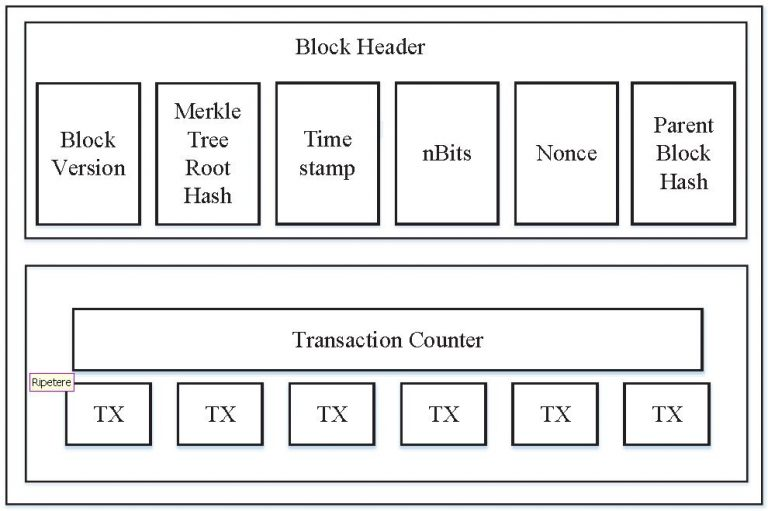
\includegraphics[width=\textwidth]{bcbl}
	\centering
	\caption{Struttura di un Blocco}
	\label{fig:blockblockchain1}
\end{figure}

Un Blocco è diviso in due parti: l`header e il body. Le transazioni sono racchiuse nel body del blocco e nell'header sono presenti i campi di gestione del blocco stesso come descritto nella figura \ref{fig:blockblockchain1}.

\begin{itemize}
  \item Versione del blocco: indica le regole di validazione del blocco da rispettare
  \item Merkle Tree Root Hash: valore della radice del Merkle Tree in cui sono salvate le transazioni del blocco
  \item TimeStamp: Marca temporale salvata come Timestamp UNIX che indica l`inserimento del blocco nella blockchain
  \item nBits: è la soglia target di un hash di blocco valido
  \item Nonce: è un campo il cui valore è settato dai miner cosicché l’hash del blocco calcolato sia minore o uguale al target attuale della rete(difficoltà). Dato che non è possibile prevedere la combinazione di bit che risulterebbero nell’hash voluto, numerosi valori di nonce sono calcolati fino a quando l’hash risultante rispetta i requisiti attuali della rete.
\item Parent Block Hash: segna l'hash del blocco a cui verrà agganciato
\end{itemize}

Il Body è composto da un contatore di transazioni (transaction counter) e dalle transazioni (TX). Tali transazioni vengono memorizzate e organizzate tramite un Merkle Tree: una struttura ad albero in cui le foglie contengono i digest hash delle informazioni mentre i nodi contengono i digest hash dei nodi sottostanti (figli).
\begin{figure}[h]
	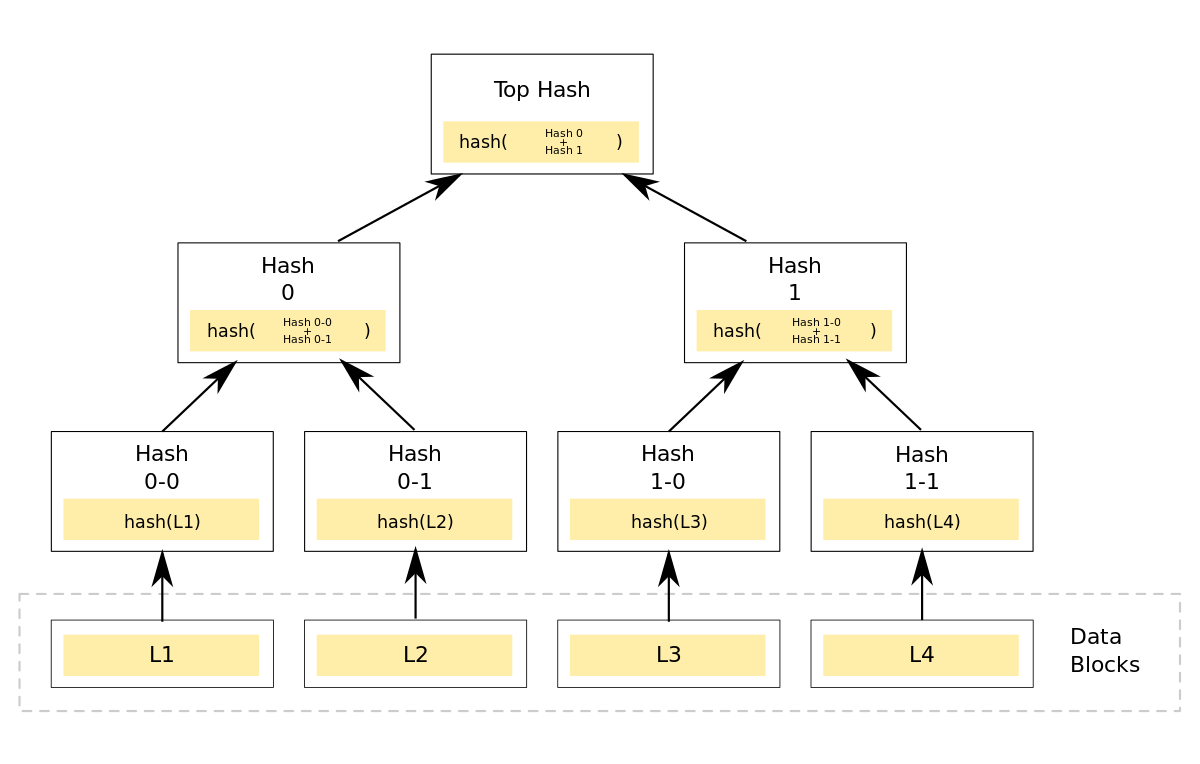
\includegraphics[width=\textwidth]{Hash_Tree}
	\centering
	\caption{Merkle Tree}
	\label{fig:Tree1}
\end{figure}

\section{Mining e Meccanismi del consenso}
I miner sono i nodi partecipanti alla rete che  ascoltano le transazioni inviate, verificano che non siano malevole e compongono un blocco organizzando le transazioni in un Merkle Tree.
I minatori che "calcolano" un blocco valido vengono premiati con un incentivo (Es: criptovaluta).
È anche possibile che più miner producano lo stesso blocco e la scelta del blocco da seguire per la catena spetta al meccanismo del consenso cioè il set di regole che permette la finalizzazione delle transazioni e il funzionamento del sistema cosicché tutti i nodi della rete convergano ad una sola versione condivisa della catena, questo andrà a creare una biforcazione o Fork da cui si avranno una sequenza valida e una sequenza orfana (o anche un singolo nodo) (Figura \ref{fig:blockchain1}).

\subsection{Consenso Trustless}
La blockhain è considerata Trustless, letteralmente "senza fiducia" poiché a differenza di un sistema centralizzato non esiste nessun ente centrale in si ripone la fiducia (come ad esempio una Banca, governi o istituti finanziari). Utilizzando un sistema decentralizzato, la fiducia non viene eliminata definitivamente ma viene suddivisa tra tutti i partecipanti, in questo modo più sarà alto il numero dei partecipanti meno fiducia si dovrà affidare ad ogni singolo nodo. %La fiducia viene riposta nei singoli nodi e che questi rispettino le regole considerate valide.

\subsection{Proof of Work}
L'algoritmo del consenso più famoso e utilizzato (come da Bitcoin, Ethereum e Monero), nonché il primo algoritmo del consenso mai creato, è il PROOF OF WORK abbreviato PoW. Questo si basa sulla "Prova del Lavoro" svolto dai miner che dovranno risolvere una serie di operazioni considerate come un puzzle matematico per poter creare un blocco valido. Il primo miner che costruisce il blocco lo aggiunge alla catena, notifica in broadcast il resto della rete e di conseguenza tutte le transazioni in esso presenti vengono validate, infine il miner viene ricompensato con un incentivo, ad esempio una moneta che sarà relativa a quello che gli utenti pagano per effettuare le transazioni, cioè le "tasse" - fees. I miner quindi utilizzano la loro potenza e risorse computazionali per provare che hanno svolto del lavoro (questo produce anche un massivo consumo di elettricità), talvolta è possibile che due o più nodi producano lo stesso blocco creando un fork e quindi due differenti catene. Il sistema è incentivato a scrivere nuovi blocchi sulla catena più lunga così da eliminare la biforcazione orfana e ricondurre tutta la rete a un`unica catena, questo implica che, se si voglia creare un blocco "falso" e farlo accettare dalla blockchain bisognerà possedere una potenza di calcolo maggiore di tutta la rete. Il mining diventa sempre più competitivo con una partecipazione sempre maggiore di persone e con un relativo incremento della difficoltà, perciò si è vista la creazione delle Mining Pool: un insieme di persone che raggruppa la propria potenza di calcolo per il mining di criptomoneta, in questo modo la probabilità di costruire un blocco valido aumenta e di conseguenza aumenta anche il guadagno suddiviso tra i partecipanti.

\subsection{Proof of Stake}
\begin{figure}[h]
	
\includegraphics[width=\textwidth]{pow-pos}
	\centering
	\caption{PoW-PoS}
	\label{fig:pow-pos}
\end{figure}

Nel 2011 basandosi sui problemi del PoW come il dispendio di energia elettrica o la creazione di grosse Mining Pool, che eliminano la decentralizzazione, si è sviluppata l`idea del PoS - Proof of Stake. Il PoS sostituisce i miner con i validatori o coniatori, questi, per far si che il loro blocco venga considerato valido devono depositare della moneta come "cauzione" chiamata Stake.
In questo modo se con il PoW era possibile inserire transazioni fraudolente, con il PoS si andrebbe a perdere la somma congelata. Il criterio di scelta dei validatori si basa sulla quantità di moneta bloccata e la durata del blocco, con il secondo parametro si va in contro al problema generato dal primo parametro cioè che solo i più ricchi possono essere scelti e quindi diventare più ricchi.
L’elezione del blocco leader (da aggiungere) avviene tramite l’algoritmo VRF – Verifiable Random Function che utilizza l’algoritmo “follow-the-coin” - “più denaro blocchi più hai fiducia”. Il PoS porta molteplici vantaggi rispetto al PoW come un minimo dispendio energetico e una maggiore sicurezza e decentralizzazione dovuta all`assenza di mining pool.

\subsection{Proof of Authority}
\begin{wrapfigure}{l}{0.5\textwidth}
	
\includegraphics[height=0.3\textheight]{judge}
\end{wrapfigure}
Un ultimo algoritmo del consenso è il PoA - Proof of Autority. Qui viene meno il concetto di decentralizzazione in quanto si basa sull'utilizzo di nodi validatori noti. Il PoA viene spesso utilizzato in ambito privato o militare e si utilizza, come intuibile dal nome, il concetto di Autorità che quindi avrà il potere di decidere i nodi validatori, cioè gli unici nodi che potranno produrre blocchi, mentre gli altri nodi avranno soltanto la possibilità di lettura. Il PoA fa si che i nodi validatori mettano in "Stake" la loro reputazione a differenza di una moneta. Il modello Proof of Authority consente alle imprese di mantenere la propria privacy e allo stesso tempo avvalersi dei vantaggi della tecnologia blockchain. Il modello PoA riduce il problema del consumo in quanto diventa inutilizzabile il concetto di concorrenza nel mining e di conseguenza le mining pool. Riferendosi al Trilemma della scalabilità, PoA rinuncia alla decentralizzazione in favore della sicurezza.

\section{Attacchi}
Nonostante la blockchain stia avendo molteplici riscontri positivi negli ultimi anni, la sua caratteristica di decentralizzazione la rende si più affidabile rispetto ad un sistema centralizzato ma risultano comunque possibili e attuabili degli attacchi ad essa.

\subsection{Selfish Mining Attack}
\begin{figure}[h]
	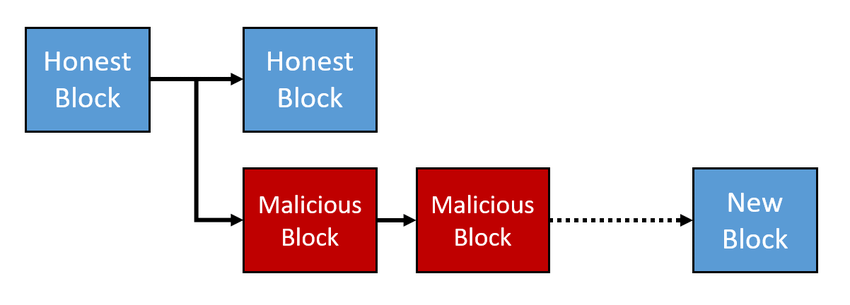
\includegraphics[width=\textwidth]{Selfish-mining-attack}
	\centering
	\caption{Selfish-mining-attack}
	\label{fig:SM-attack}
\end{figure}
Il Selfish Mining Attack si basa su un sistema PoW e sfrutta la sua debolezza nel momento in cui si genera una Fork. Nel momento in cui si genera una biforcazione solo la catena più lunga viene considerata valida e le transazioni nella catena orfana vengono rese nulle. Per l`attuarsi del Selfish Mining Attack si ha bisogno che l`attaccante cioè il Fault-Miner generi un blocco che potrebbe creare una Fork (in cui si ha la possibilità di inserire transazioni fraudolente) ma lo tenga segreto, senza aggiungerlo alla Blockchain. Il Fault-Miner dovrà continuare a generare blocchi seguendo la sua catena e quando questa sarà più lunga di quella che attualmente gli altri miner stanno seguendo, pubblicherà la sua Fork e la sua catena che essendo più lunga, secondo l`algoritmo del PoW verrà considerata valida e sarà quella che gli altri miner seguiranno da quel momento in poi. Per l`attuazione del Selfish Mining Attack si ha bisogno quindi che un singolo ente possegga più del 51\% della potenza dell`intera rete.

\subsection{Double Spending Attack}
\begin{figure}[h]
	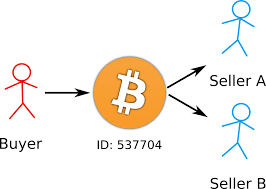
\includegraphics[height=0.2\textheight]{dsa}
	\centering
	\caption{Double Spending Attack}
	\label{fig:ds-attack}
\end{figure}
Il Double Spending Attack viene concepito per la possibilita di spedere due volte la stessa moneta. Questo potrebbe essere attuabile con la creazione di due diverse transazioni. Le due transazioni però dovranno appartenere a due blocchi diversi. E se due miner che competono nel minare un blocco utilizzano ognuno una transazione diversa? Allora verranno prodotti due blocchi con entrambe le transazioni ma verrà prodotta una Fork quindi solo una delle due transazioni verrà poi validata mentre la seconda sarà annullata, ricordando che una transazione o meglio un blocco ha una validità pari al numero di blocchi minati in seguito (In BitCoin un blocco è validato se sono stati prodotti 6 blocchi successivi).

\section{Blockchain Pubbliche/Private}
Una blockchain pubblica solitamente è anche detta permissionless, letteralmente "senza permessi" cioè un nuovo nodo non ha bisogno di speciali permessi per partecipare, quindi minare o effettuare transazioni nella rete che viene definita pubblica. Le reti permissionless sono quindi decentralizzate in quanto nessuno ha il controllo della rete.

Le blockchain private sono conosciute come permissioned, sono caratterizzate dalla presenza di un’autorità centrale che decide chi può accedere e assegna loro un ruolo nella rete che determinerà cosa il nuovo nodo avrà il permesso di fare, se ha la possibilità di partecipare alla rete o se potrà essere un nodo validatore o di sola lettura. La sicurezza di una blockchain privata fa maggiormente perno sull'affidabilità dei singoli partecipanti.

\section{Ethereum}

\begin{figure}[h]
	
\includegraphics[height=0.2\textheight]{eth}
	\centering
	\caption{Etherium Logo}
	\label{fig:eth-logo}
\end{figure}

Ethereum è una piattaforma decentralizzata ideata nel 2013 (in seguito pubblicata nel 2015) come sostituto a BitCoin. Ethereum è una piattaforma basata su blockchain che permette la gestione di smart contract e, come Bitcoin, mette a disposizione una moneta che viene analogamente chiamata Ether e abbreviata con ETH. La moneta viene utilizzata per le varie transazioni ma viene anche usata per pagare le "tasse" - fees, nello specifico viene utilizzato un sottomultiplo dell'ETH chiamato wei che corrisponde a circa  $ 10^{-18} $ ETH  ( 1 ETH = $ 10^{18} $ wei). Per lo sviluppo e l'interfacciamento viene messa a disposizione da Ethereum la EVM - Ethereum Virtual Machine che funge da macchina turing completa in grado di eseguire byte code. La sua funzione è quella di consentire l'esecuzione di programmi o smart contract al fine di implementare una serie di funzionalità aggiuntive su detta blockchain; la EVM utilizza per gli smart contract un linguaggio di alto livello specializzato chiamato Solidity.

\subsection{Smart Contract}
\begin{wrapfigure}{l}{0.4\textwidth}
	\includegraphics[height=0.2\textheight]{SmartC}
	\centering
\end{wrapfigure}

Uno Smart Contract, o contratto intelligente, è un programma messo a disposizione da ethereum e consiste in una collezione di codice (funzioni) e di dati (stato). Lo smart Contract è identico ad un contratto reale ma grazie alla tecnologia blockchain non necessita di un terzo ente verificatore. Essi sono programmi scritti in un linguaggio di programmazione ad alto livello come Solidity (simil-JavaScript) o Vyper (simil-Python), compilati in bytecode e distribuiti sulla blockchain tramite speciali transazioni inviate ad un generico indirizzo 0x0 pagando un determinato gas. Nonostante siano caricati da un utente, gli smart contract non hanno un proprietario ma appartengono alla rete, anche la loro sicurezza deriva da essa e vengono infatti definiti come programmi "on-chain" cioè programmi caricati su rete che mantengono uno stato sicuro e inviolabile al di fuori delle regole del contratto stesso infatti, una volta caricato, non può essere modificato. Ogni operazione, gestita da uno smart contract, che si vuole effettuare comporta una transazione che avrà come destinatario l'indirizzo del contratto e come una qualunque transazione sarà considerata valida solo una volta che la rete l'avrà validata.

\subsection{Solidity}
Solidity è il linguaggio più diffuso nel contesto Ethereum ed è un linguaggio orientato agli oggetti, compilato, staticamente tipato e di alto livello usato per implementare smart contract eseguibili sull’Ethereum Virtual Machine. È stato sviluppato per essere simile alla sintassi ECMAScript per renderlo familiare agli sviluppatori web. Solidity è un linguaggio fortemente tipato, i tipi delle variabili sono gestiti in modo statico, cioè il tipo va dichiarato nel momento in cui questa viene creata. Solidity gestisce i tipi di dato in tre suddivisioni:
\begin{itemize}
  \item Tipi Valore: possono essere utilizzati per lo storage di comuni valori come un INT oppure UINT per un unsigned int, ma vengono considerati tali anche i bool o le string;
  \item Tipi indirizzo: come specificato dal nome indicano gli address di altre variabili/oggetti;
  \item Tipi mapping: rappresentano strutture dati di tipo chiave/valore. Durante la creazione tutti i valori vengono inizializzati con i byte a zero, il loro uso è analogo ad un "array" visto da altri linguaggi o meglio ad una HashMap.
\end{itemize}
Le funzioni rappresentano il codice eseguibile di uno smart contract, possono prendere vari parametri in input e possono restituire più argomenti come output che andranno specificati nella firma. Queste posseggono una visibilità che può essere public, private, external, internal.
Un contratto di esempio :
\begin{lstlisting}[language=Solidity]
pragma solidity >=0.4.0 <0.6.0;
contract SimpleStorage {
 uint storedData;

 function set(uint x) public {
 	storedData = x;
 }
 function get() public view returns (uint) {
 	return storedData;
 }
}
\end{lstlisting}
Nella prima riga si nota la dicitura pragma solidity che indica la versione del linguaggio utilizzata per scrivere il contratto che quindi indica al compilatore la versione da utilizzare per una giusta compilazione. In seguito inizia la definizione del contratto. Questo possiede una variabile storedData di tipo Unsegned Int di 256bit, e due funzioni con visibilità pubblica, la prima set ha un argomento di tipo uint e nessun return mentre nella seconda viene (nella firma) segnato il return e il tipo restituito (uint).

\subsection{Gas}
Quando si effettua una transazione o si carica uno smart contract la EVM richiede un pagamento calcolato in gas. Il gas è una frazione dell'ether e viene richiesto per un'operazione come l'invio di una transazione, viene comunemente chiamato "transaction fee". Il gas viene anche richiesto quando si effettua una qualunque operazione tramite uno smart contract ed è calcolato in base alla complessità di questa e da quanta memoria si va a utilizzare. 

\subsection{DApps}

Le DApps - Decentralized APPlications sono applicazioni simili alle app tradizionali, con la differenza fondamentale che al posto di appoggiarsi su server centralizzati sfruttano le piattaforme blockchain e il loro network distribuito, in questo modo possono essere utilizzate da interfaccia con gli smart contract. Le DApp sono immutabili, quindi nessuno può modificare quello che avviene tramite l’applicazione.

%capitolo 3
\chapter{Tecnologie utilizzate}

\section{Hyperledger Besu}
\begin{wrapfigure}{r}{0.4\textwidth}
	
\includegraphics[height=0.2\textheight]{Hyperledger_Besu}
	\centering
	\caption{Hyperledger Besu logo}
	\label{fig:Hyperledger_Besu_logo}
\end{wrapfigure}

Hyperledger è un open source creato per far progredire le cross-industry blockchain technologies. Si tratta di una collaborazione globale, ospitata da The Linux Foundation, che include leader in finanza, banche, IoT, supply chain, manufacturing e tecnologia.

Hyperledger Besu è un Ethereum client - open source sviluppato sotto Apache 2.0 e scritto utilizzando Java. Può essere utilizzato per la rete pubblica Ethereum oppure per una rete permissioned privata, viene anche utilizzata per le reti di test come Rinkeby, Ropsten, and Görli. Hyperledger Besu include molti algoritmi del consenso tra cui PoW e PoA (IBFT, IBFT 2.0, Etherhash, and Clique).

Hyperledger Besu offre molte proprietà tra cui una EVM completa che permette l'invio e l'esecuzione di smart contract con  transazioni su Ethereum blockchain. 

Besu usa un RocksDB key-value database per la persistenza locale dei dati della rete. I dati si dividono in due categorie:
\begin{itemize}
\item Blockchain: I dati della blockchain sono composti dal Block Header che forma la "catena" di dati utilizzata per verificare crittograficamente lo stato blockchain, block bodies che contengono la lista delle transazioni ordinate comprese in ciascun blocco e ricevute di transazione che contengono metadati relativi all'esecuzione della transazione, inclusi i transaction logs.
\item World State: Il world state è un mapping da addresses to accounts
\end{itemize}

Hyperledger Besu implementa Ethereum’s devp2p network protocols per l'inter-client communication e un altro sotto-protocollo per l'IBFT 2.

Hyperledger Besu mette a disposizione del programmatore le API di EEA e JSON-RPC utilizzando protocolli HTTP e WebSocket.

Hyperledger Besu permette di monitorare i nodi e la performance della rete, i nodi sono monitorati usando Prometheus o le metriche di debug JSON-RPC API method, invece la performance della rete viene monitorata con un qualunque Block Explorer.

\subsection{IBFT} \label{IBFT}
Un meccanismo di consenso messo a disposizione da Besu (e sarà anche quello utilizzato nello sviluppo della blockchain) è l'IBFT versione 2.0 basato su PoA (Proof of Authority), questo è un protocollo utilizzabile solo dalle reti private. Nelle reti IBFT 2.0 solo i nodi pre-approvati, conosciuti come validatori, possono validare transazioni e blocchi. I validatori prendono un turno per creare il prossimo blocco; prima che questo venga inserito sulla catena la maggioranza dei validatori (maggiore del 66,6\%) deve prima firmare il blocco. Per aggiungere o rimuovere un validatore si ha, anche qui, bisogno della maggioranza dei voti; IBFT 2.0 ha bisogno di minimo 4 nodi per essere Byzantine Fault Tolerant, ciò consiste nell'abilità per una rete blockchain di funzionare correttamente e di raggiungere il consenso nonostante i nodi falliscano o propaghino informazioni errate ai peer.

Per usare IBFT 2.0, Besu richiede la scrittura di un genesis file (file contenente le configurazioni necessarie alla rete)
\begin{lstlisting}[language=json,firstnumber=1]
"config": {
	"chainId": 1981,
	"muirglacierblock": 0,
	"ibft2": {
		"blockperiodseconds": 2,
        "epochlength": 30000,
        "requesttimeoutseconds": 4,
        "blockreward": "5000000000000000",
        "miningbeneficiary": "0xfe3b557e8fb62b89f4916b721be55ceb828dbd73"
    }
}
\end{lstlisting}
Riferendosi al codice di esempio sopracitato (genesis file) si vedono i dati di config di una rete ibft2 identificando:
\begin{itemize}
\item blockperiodseconds: anche chiamato block time, è il tempo alla cui scadenza il protocollo propone un nuovo blocco;
\item epochlength: numero di blocchi che indica ogni quanto resettare i voti;
\item requesttimeoutseconds: il timeout in secondi di un round per il cambio di validatore;
\item blockreward: importo della ricompensa opzionale in Wei per premiare il beneficiario;
\item miningbeneficiary: il beneficiario opzionale del blockreward.
\end{itemize}

\subsubsection{IBFT Methods / Besu API}
Besu per la gestione dell'IBFT offre delle API sviluppate per mezzo di metodi utilizzabili tramite chiamate post. Tra i più utilizzati / quelli necessari c'è \textit{ibft\_discardValidatorVote} che prende in input l'indirizzo di un nodo e restituisce un booleano analogo al fine dell'operazione, con questo metodo è possibile rimuovere da un nodo la proprietà di validatore se più del 50\% della rete effettua questo voto. Analogamente si usa \textit{ibft\_proposeValidatorVote} per proporre un nuovo nodo come validatore. Infine ci sono molteplici metodi per ottenere delle metriche come \textit{ibft\_getValidatorsByBlockHash} e \textit{ibft\_getValidatorsByBlockNumber} che restituiscono la lista di validatori che hanno firmato un blocco a partire dal suo hash o il numero del blocco.

\subsection{Free Gas Network}\label{free-gas-network}
Con Free Gas Network ci riferiamo ad una rete in cui vengono annullate le tasse "fee" delle transazioni. Utilizzando un client ethereum come BESU le tasse vengono calcolate tramite il gas e il prezzo che ha un'unità di esso: il costo di una transazione è quindi  gas used * gas price. Utilizzando il comando \textit{--min-gas-price=0} all'avvio di Besu il gas price impostato a zero, in questo modo il gas richiesto da una transazione verrà reso nullo in quanto il valore di questo sarà zero (gas x 0 = 0), quindi tutti i nodi potranno effettuare transazioni senza pagare alcuna tassa.

%\subsection{API Methods}
\section{Truffle}
Truffle è il framework più utilizzato per lo svilupo su Etherieum e permette il management degli smart contract per tutto il loro ciclo di vita. L'installazione di Truffle avviene tramite il comando
\begin{lstlisting}[language=command.com]
npm install truffle -g
\end{lstlisting}
che fa uso del gestore di pacchetti npm.
Una volta installato è possibile inizializzare un progetto tramite 
\begin{lstlisting}
truffle init
\end{lstlisting}
una volta creata la nuova directory avrete la seguente struttura:
\begin{lstlisting}[language=command.com]
contracts/: Directory per i contratti sviluppati con Solidity
migrations/: Directory per i file di deploy
test/: Directory per i file di test degli  smart contract
truffle-config.js: Truffle configuration file
\end{lstlisting}

\subsection{Compile}
Con la Truffle suit è possibile compilare i propri smart contract. Con il comando 
\begin{lstlisting}[language=command.com]
truffle compile
\end{lstlisting}
verranno compilati i contratti, quindi si avrà una visione dei possibili errori oppure, se compilati correttamente, verrà generata per ogni contratto la sua ABI - Application Binary Interface, queste sono scritte tramite modello JSON, avranno lo stesso nome del contratto e saranno nella directory \textit{build/contract}.

\subsection{Test}
Con Truffle è possibile scrivere ed eseguire dei test per i contratti. Tali test andranno scritti in JavaScript, firmati con estensione \textit{.spec.js} e salvati nella directory \textit{/test}.
Con il comando
\begin{lstlisting}[language=command.com]
truffle test
\end{lstlisting}
vengono eseguiti i vari programmi sulla rete di test e verrà visualizzato su riga di comando quali di questi sono andati a buon fine e quali hanno generato dei problemi che verranno mostrati.

\subsection{Deploy}
All'avvio di truffle init viene creato un file nominato truffle-config.js - file formato json che contiene le configurazioni di Truffle. Inizialmente sarà vuoto ma, specificando una qualunque rete, Truffle ci permette di effettuare il deploy / migration dei nostri smart contract sulla rete selezionata scrivendo il file di migration (uno per ogni contratto) ed eseguendo il comando
\begin{lstlisting}[language=command.com]
truffle migrate --network=//nome-rete
\end{lstlisting}

\section{Node.js}

Node.js è una tecnologia open source di sviluppo software, orientata agli eventi per l'esecuzione di codice JavaScript costruito su Google Chrome’s V8 JavaScript engine.
\begin{figure}[h]
	
\includegraphics[height=0.15\textheight]{node-js}
	\centering
\end{figure}
È un linguaggio event-driven, usa la programmazione asincrona, non supporta il multithreading e il modello di programmazione si basa sulle funzioni di callback cioè funzioni che andranno in esecuzione solo dopo che è stato lanciato l'evento, il quale indica che l'elaborazione è terminata e il valore di output è disponibile.
Questo ambiente ci permette di utilizzare il linguaggio JavaScript sia front-end sia back-end, rendendo possibile la creazione di un server tramite l'uso di pacchetti come Express che sarà in ascolto di default sulla porta 1010:
\begin{lstlisting}[language=JavaScript]
const express 		= require('express');
const app = express();

app.get('/', (req, res) => {
  	//codice
});
\end{lstlisting}

\subsection{Web3}

Web3 è una collezione di librerie che permette la connessione con un nodo Ethereum locale o remoto. Web3 viene utilizzata come una classica libreria JavaScript caricata tramite la KeyWord \textit{require} di Node.js : 
\begin{lstlisting}[language=JavaScript]
var Web3 = require('web3');
\end{lstlisting}
in seguito deve essere inizializzata con un argomento di tipo stringa che rappresenta l'indirizzo del nodo Ethereum a cui collegarsi:
\begin{lstlisting}[language=JavaScript]
var web3 = new Web3(Web3.givenProvider || 'local-or-remote-address:8546');
\end{lstlisting}

%capitolo 4
\chapter{Caso d'uso}

\section{Problema Iniziale}
Il progetto blockchain è stato ideato e sviluppato come proposta di soluzione ai problemi nella gestione del tracciamento, invio, certificazione e mantenimento di dati riguardanti "spostamenti". Questi spostamenti sono informazioni (LOG) inviate da un qualunque ente che metta a disposizione della società un servizio che preveda dei mezzi pubblici o privati quali ad esempio autobus, treni, taxi, etc. Ad oggi queste informazioni vengono raccolte, analizzate e utilizzate su di modelli di storage a fogli di calcolo (Ad Esempio EXCEL - Programma Microsoft). I fogli di calcolo offrono alcuni vantaggi come la semplicità con cui vengono creati, scritti e salvati benché offrano un'interfaccia poco user friendly ('facilmente utilizzabile') guardando tutti i possibili attori. Il progetto si focalizza sui difetti come la pubblicazione/condivisione delle informazioni o l'interrogazione di queste in quanto, utilizzando semplici fogli, non esistono regole di struttura e organizzazione, e si pone particolare importanza alla sicurezza e all'affidabilità di queste informazioni e che non vengano modificate durante la condivisione, quindi la possibile certificazione di esse.

\section{Soluzione}
La soluzione proposta si offre di risolvere tutti i problemi sopra elencati come certificazione, salvataggio e interrogazioni di informazioni. Viene ideata una blockchain privata che avrà funzione di ente (decentralizzato) certificatore. Questa non utilizza nessuna moneta creando una Free Gas Network e con l'ausilio di appositi smart contract (scritti e caricati autonomamente) ci permette di salvare un codice che andrà ad identificare un determinato gruppo di spostamenti come un codice Hash che usufruendo della struttura e utilizzo della blockchain non potrà essere modificato. Ciò implica che si potrà sempre verificare la correttezza del gruppo di spostamenti richiesti ricreando e controllando il loro codice.

La memorizzazione dei dati viene invece affidata ad un database relazionale, utilizzando nel progetto il DBMS (Database Managenent System) MySql, che ci permette di salvare grandi quantità di dati con una efficiente organizzazione gestita con la creazione di tabelle così da essere facilmente interrogabile in futuro.
 
L'interfaccia comune è gestita con un server sviluppato tramite tecnologia Node.js che con una Single Page Application avrà la funzione di interfaccia user friendly. Avrà funzioni di: memorizzazione per i log degli spostamenti su Database, calcolo e salvataggio dei loro codici hash sulla blockchain al tempo stimato e quando necessario. Nel momento in cui verranno richiesti dei dati e avverrà l'interrogazione del Database sarà reso obbligatorio il controllo di questi con il codice sulla blockchain. Inserendo questo WebServer intermedio o server proxy si andrà ad eliminare il passaggio di dati non propriamente protetto, rendendo partecipi tutti i singoli attori dell'attività.

\subsection{Problematiche}
Utilizzando delle nuove tecnologie sorgono comunque nuove problematiche che non sono state affrontate nello sviluppo in quanto non inerenti ai fini del progetto.

%DOS utilizzando un solo server
Una prima problematica si sviluppa utilizzano un server proxy. Avendo un singolo server di accesso al database e alla blockchain, se questo non viene correttamente protetto e costantemente controllato è soggetto ai classici attacchi come un DDOS - Distributed Denial of Service in cui si utilizzano molteplici messaggi fittizi (come un inizio di HandShake per una connessione TCP) per far si che il server non possa sostenere tutti i servizi ed essendo l'unico punto di accesso bloccherebbe il funzionamento della rete blockchain.

%blockchain utile solo con molti nodi
Una caratteristica che rende sicura la blockchain pubblica è la molteplicità di nodi, questa con una blockchain privata, come la nostra, va a decadere con il discendere  del numero di nodi; utilizzando un meccanismo di consenso basato su PoA (Proof of Autority) si ha infatti bisogno di un minimo di 4 nodi per essere resistente al problema bizantino.

%attacco del compleanno
Per evitare l'appesantimento della Blockchain si è pensato di salvare su di essa solo un codice identificativo (codice Hash) per un gruppo di Log. Questo implica che con l'aumentare dei log identificati da un singolo codice hash diminuisca la sicurezza che questo apporta, infatti, sarà più facilmente utilizzabile un attacco come l'attacco del compleanno che ha come obiettivo quello di generare una collisione. Questo ha l'obiettivo di trovare dei dati fittizi ai Log originari che però generano lo stesso codice Hash, questi dati fittizi potranno essere quindi sostituiti nel DB ma verranno comunque considerati certificati dal sistema in quanto produrranno lo stesso codice.

\section{Attori}
Il caso d'uso per il progetto blockchain prevede la partecipazione di diversi attori quali: 

Un Terminal User o utente finale, è un comune dipendente di un ente che partecipa alla blockchain il quale ha il compito di comunicare i propri spostamenti/Log o qualunque informazione di cui si preveda il salvataggio;

Un Admin uno dei dipendenti di enti partecipanti che viene segnato dagli stessi come amministratore e che quindi possiede  particolari oneri come il possesso e la trasmissione di una chiave privata;

Il proprietario/gestore della blockchain avrà il compito di gestire l'intera blockchain privata con l'amministrazione che ne segue, come la supervisione dei nodi presenti, il loro funzionamento e la loro caratterizzazione come validatori. 

\section{Scenario di utilizzo}
Il Progetto prevede uno scenario di utilizzo diverso seguendo la distinzione degli attori.
Per l'utilizzo si prevede che ad ogni ente partecipante al progetto venga assegnato un account, cioè una coppia di chiavi, privata e pubblica, che serviranno per interagire con la blockchain, inoltre ogni ente dovrà inserire i propri dipendenti nel Database e specificare il ruolo di essi, se Admin o Terminal User.

Un Terminal User, una volta effettuato l'accesso, viene portato ad un'interfaccia in cui può inserire la città che sarà selezionata come Start dello spostamento e in seguito viene spostato in una seconda interfaccia da cui può terminare lo spostamento o annullarlo, se annullato potrà cominciare un nuovo spostamento dalla precedente interfaccia. Il completamento di questo avverrà solo se compila i campi necessari quali la città di Termine e la distanza percorsa indicata in Kilometri.

Un Admin, una volta effettuato l'accesso, potrà, a differenza di un Terminal User, effettuare delle query/interrogazioni riguardo gli spostamenti compiuti. Inserendo una data otterrà tutti gli spostamenti che sono stati certificati da una transazione inserita in quella determinata data, da qui potrà anche accedere ai dettagli della transazione o del blocco che la contiene riferendosi alla blockchain, inoltre, quando il sistema lo richiede, ha il compito di inserire la Private Key dell'utente (ente) che verrà utilizzata per la scrittura su blockchain.

%capitolo 5
\chapter{Sviluppo}
\section{Schema Progetto}\label{Schema-Progetto}
Il Progetto è stato ideato partendo dalla ben conosciuta architettura client-server dove però è stata implementata anche la tecnologia blockchain. Come identificabile nella figura \ref{fig:sch} esistono 2 grandi attori; i "client" mostrati come dei mezzi di trasporto (Autobus-Taxi-Treni) hanno il compito/funzione di inviare i dati raccolti riguardanti gli spostamenti, in generale possiamo identificare questi dati come: 
\begin{itemize}
\item Città di partenza;
\item Città di arrivo;
\item Distanza percorsa;
\item Data della percorrenza (identificata nel progetto come la data di Partenza e data di Arrivo);
\item Username dell'utente che ha svolto la tratta;
\end{itemize}
nello schema \ref{fig:sch} sono descritti in modo convenzionale come Msg("A .to. B") (Message).
\begin{figure}[h]
	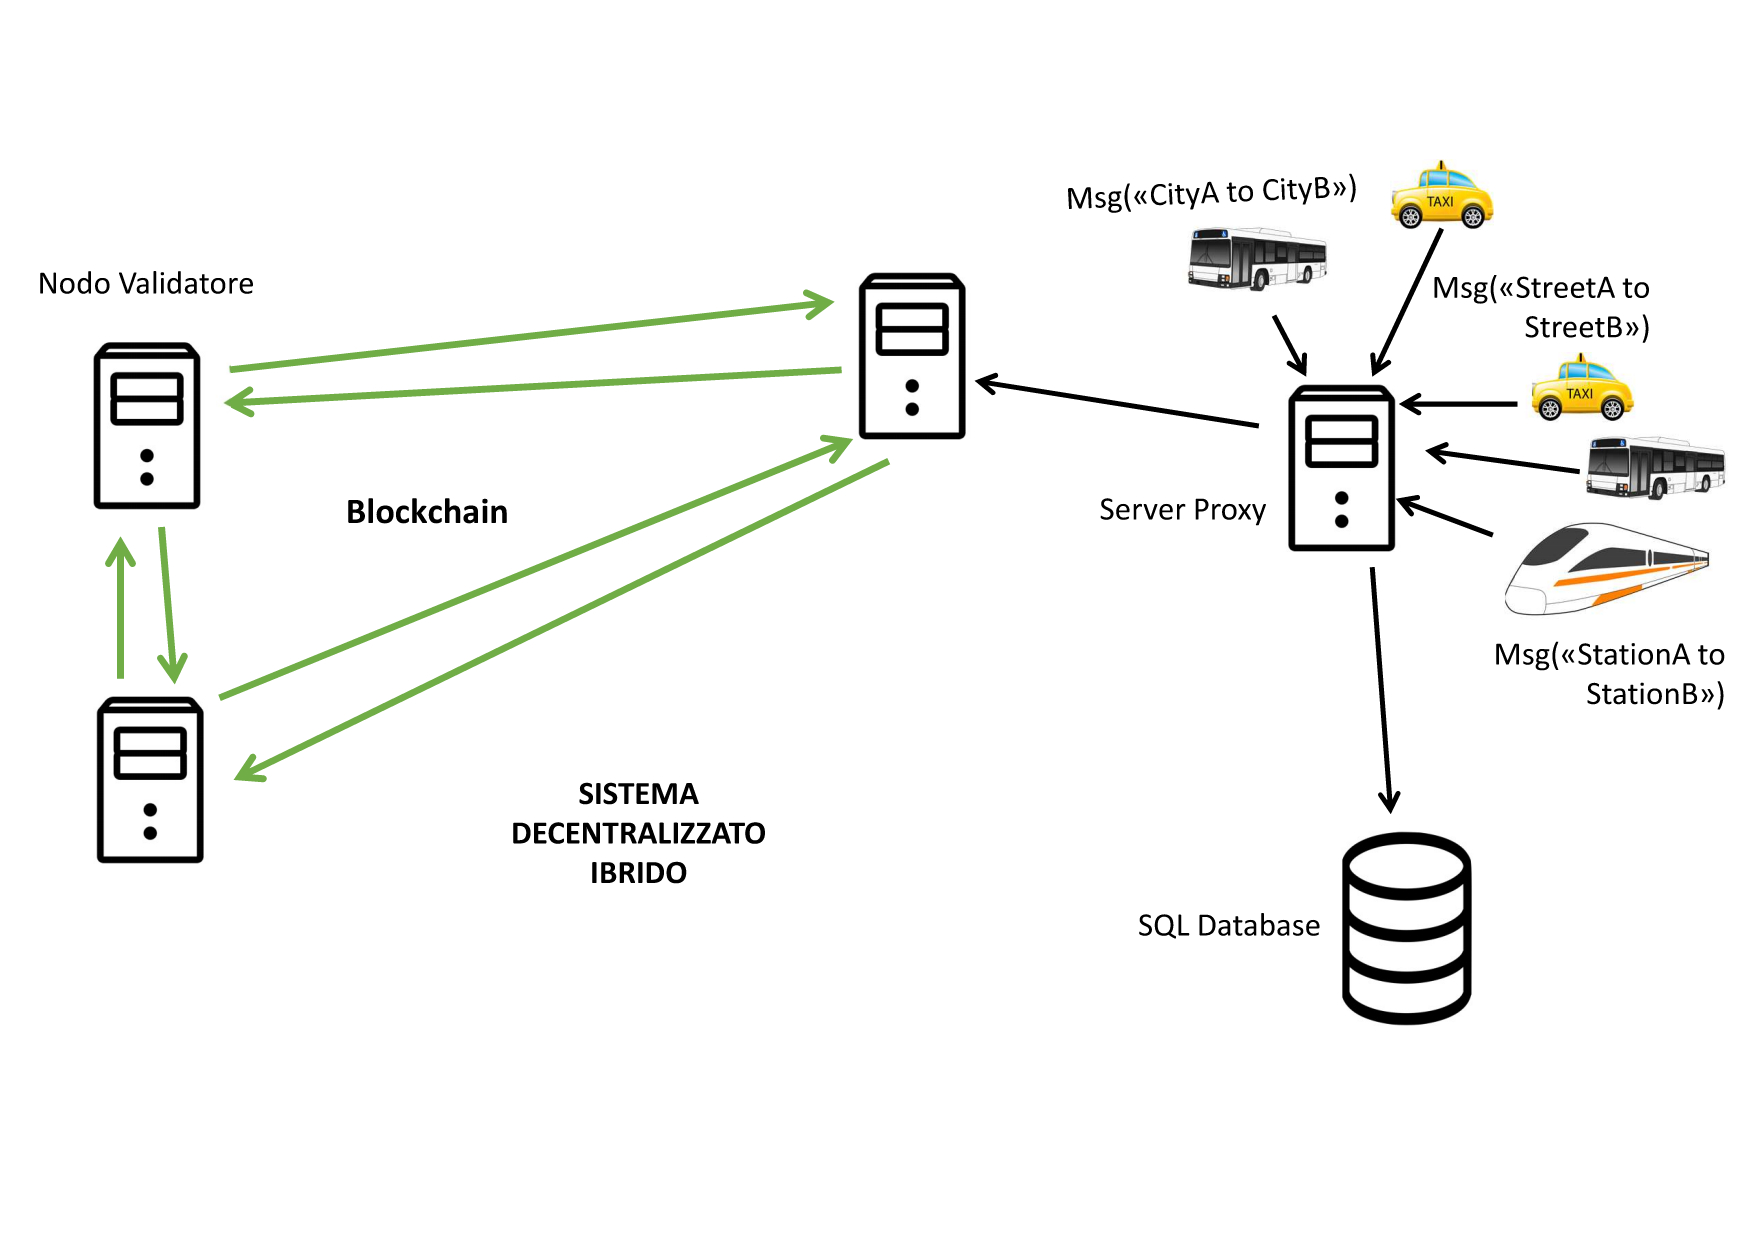
\includegraphics[width=\textwidth]{Schema_Progetto}
	\centering
	\caption{Schema generale del progetto}
	\label{fig:sch}
\end{figure}

Questi vengono inviati al secondo attore dello schema \ref{fig:sch}, il server Proxy. Questo ha lo specifico compito di ricevere ed elaborare in modo opportuno i diversi dati. Il server proxy ha una duplice funzione di interfaccia, con il database e con la blockchain, funge quindi da ponte tra le due strutture.

\section{Blockchain Ibrida}
Il progetto è incentrato su due strutture di immagazzinamento dati, questo rende possibile l'utilizzo dei vantaggi di entrambi.

La blockchain è sviluppata con BESU eseguendo 4 nodi (il minimo per essere BFT) avviati in locale.
Il primo passo è creare una directory da utilizzare che conterrà una directory per ogni nodo che a sua volta conterrà una directory per lo storing dei dati.
\begin{lstlisting}[language=command.com]
IBFT-Network/
		Node-1
				data
		Node-2
				data
		Node-3
				data
		Node-4
				data
\end{lstlisting}

Il secondo passo è creare un file di config per la rete (descrizione nel capitolo ~\ref{IBFT}).
Come terzo passo si ha l'esecuzione di un comando che permette la creazione delle chiavi pubbliche e private per ogni nodo, questo passo è possibile saltarlo ma in seguito si possiederà solo la chiave privata del nodo.
\begin{lstlisting}[language=command.com]
besu operator generate-blockchain-config --config-file=ibftConfigFile.json --to=networkFiles --private-key-file-name=key
\end{lstlisting}

L'ultimo passo è l'avvio di ogni singolo nodo. La blockchain si basa sull'avvio di uno o più nodi come bootnode, cioè nodi a cui gli altri nodi che si avvieranno faranno riferimento per ottenere la lista completa dei nodi partecipanti e interconnettersi con la blockchain.
Il primo nodo viene perciò avviato con queste caratteristiche:
\begin{lstlisting}[language=command.com]
besu --data-path=data --genesis-file=..\genesis.json --rpc-ws-enabled --rpc-http-enabled --rpc-http-api=ETH,NET,IBFT,WEB3 --host-allowlist="*" --rpc-http-cors-origins="all" --metrics-enabled --min-gas-price=0
\end{lstlisting}

Con le prime 2 opzioni si specifica rispettivamente il path/directory dove effettuare lo storage delle informazioni e il path del file di genesi della rete. 
\begin{itemize}
\item rpc-ws-enabled: Abilita il servizio WebSockets JSON-RPC
\item rpc-http-enabled: Abilita e quindi permette l'uso delle JSON-RPC API specificate tramite \textit{rpc-http-api}
\item host-allowlist: Abilita gli host selezionati (* = tutti) per l'accesso alle HTTP JSON-RPC API
\item rpc-http-cors-origins: abilita tutti i domini ad accedere al nodo tramite HTTP JSON-RPC API
\item metrics-enabled: Abilita le metriche / il monitoraggio dei nodi con applicativi come Prometheus o Grafana
\item min-gas-price: Imposta il prezzo del gas, permette una free gas network ~\ref{free-gas-network}.
\end{itemize}

\begin{figure}[h]
	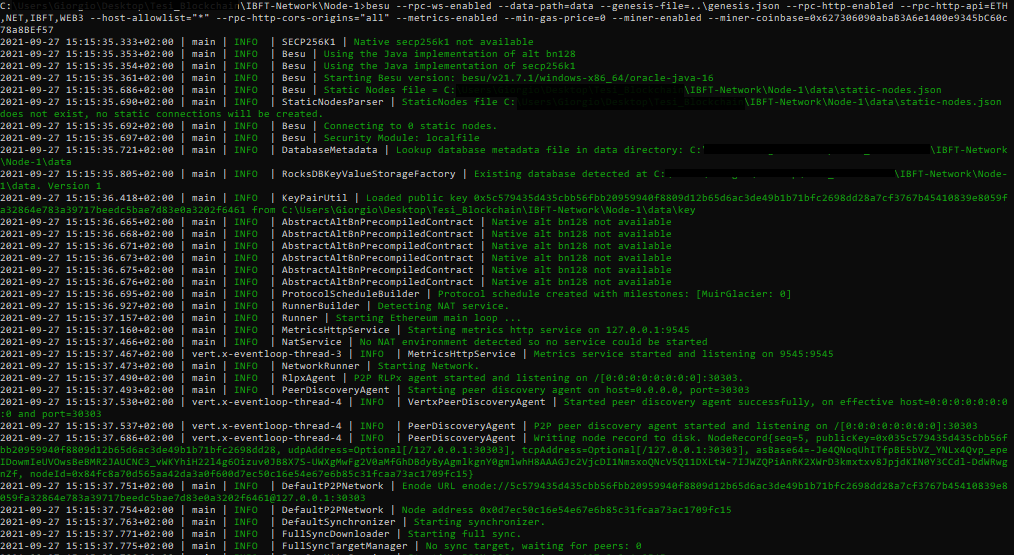
\includegraphics[width=\textwidth]{Besu-avvio}
	\centering
	\caption{Schermata avvio nodo con Besu}
	\label{fig:sch-avvio-besu}
\end{figure}

I successivi nodi saranno avviati in maniera analoga
\begin{lstlisting}[language=command.com]
besu --data-path=data --genesis-file=..\genesis.json --bootnodes=enode://5c579435d435cbb56fbb20959940f8809d12b65d6ac3de49b1b7 1bfc2698dd28a7cf3767b45410839e8059fa32864e783a39717b eedc5bae7d83e0a3202f6461@127.0.0.1:30303 --p2p-port=30304 --rpc-http-enabled --rpc-http-api=ETH,NET,IBFT,WEB3 --host-allowlist="*" --rpc-http-cors-origins="all" --rpc-http-port=8547 --min-gas-price=0
\end{lstlisting}

La principale differenza è che bisogna specificare l'address del bootnode a cui collegarsi, questo è chiamato enode address e ogni nodo ne posside uno, viene visualizzato all'avvio del nodo ed è composto da 
enode://chiave-pubblica-nodo@indirizzo-or-127.0.0.1(localhost):porta-p2p; con rpc-http-port viene specificata una porta di interfaccia al nodo, se non specificata viene utilizzata la porta di default 8545. Una volta avviato il numero minino di nodi si verificherà l'avvio della connessione tramite l'import e il producing di blocchi.
\begin{figure}[h]
	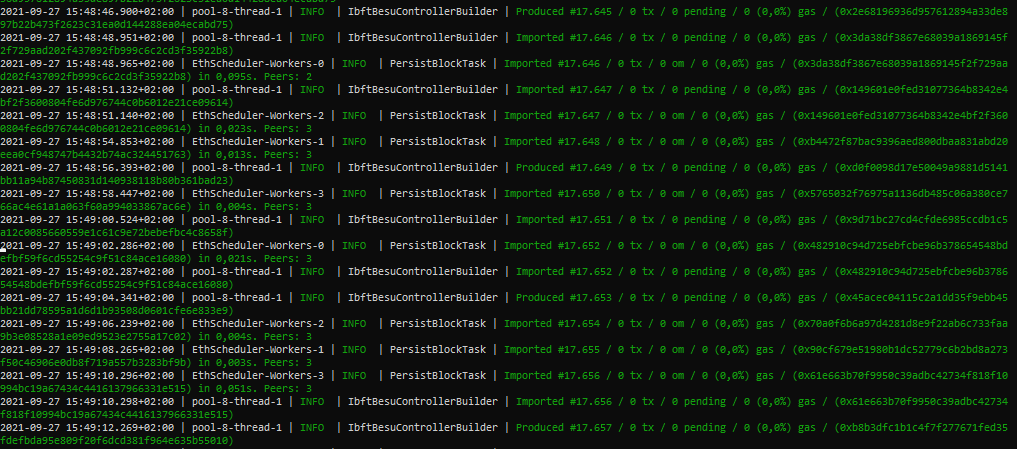
\includegraphics[width=\textwidth]{Besu-imported-produced}
	\centering
	\caption{Schermata funzionamento nodo besu}
	\label{fig:besu-imported-produced}
\end{figure}
Una volta visualizzato ciò, la blockchain sarà attiva e si potrà comunicare con essa sulle rispettive porte dei nodi con librerie come WEB3.

La seconda struttura dati è un database relazionale SQL. Avviato in locale grazie all'applicativo XAMPP che comprende 4 tabelle (Le tabelle sono state sviluppate per uno scenario di testing perciò con dati minimi).
\begin{lstlisting}[language=SQL]
CREATE TABLE ID_Hash(
	Business varchar(42) REFERENCES Business(Business_Hex),
	ID_HASH int REFERENCES Log(ID_HASH),
	Data DATETIME,
	TransactionHash varchar(255) NOT NULL,
	PRIMARY KEY (Business, ID_HASH)
);

CREATE TABLE Log(
	City_Start varchar(255) NOT NULL,
	City_Finish varchar(255) NOT NULL,
	UserName varchar(255) NOT NULL REFERENCES TerminalUser(UserName) ,
	Distance DOUBLE(8,4),
	DataStart DATETIME,
	DataFinish DATETIME,
	ID_HASH int NOT NULL,
	PRIMARY KEY (UserName, DataStart)
);

CREATE TABLE Business(
	BusinessName varchar(255) PRIMARY KEY,
	Business_Hex varchar(42) UNIQUE NOT NULL
);

CREATE TABLE TerminalUser(
	UserName varchar(64) PRIMARY KEY,
	password varchar(255) NOT NULL,
	Business_Hex varchar(42) NOT NULL REFERENCES Business(Business_Hex),
	Administrator BOOLEAN
);
\end{lstlisting}

La tabella Business indica, come descritto dal nome, una lista di aziende con un determinato nome e siccome sono aziende partecipanti al consorzio e al progetto, avranno un account sulla blockchain e verrà memorizzato in relazione al nome la loro chiave pubblica. Nella tabella TerminalUser vengono memorizzati gli utenti o dipendenti che di conseguenza possiedono dei dati per il login (Username, Password), i dati di riferimento dell'azienda e un booleano che indicherà il loro ruolo; false = ruolo normale, true = amministratore. Il riferimento agli Utenti è posseduto dalla tabella Log, atta a contenere i dati degli spostamenti  come specificato nello schema ~\ref{Schema-Progetto}, questi inoltre possiedono un ID\_HASH, cioè un id che raggruppa determinati log, questo id fa da tramite/identificativo con la blockchain in quanto l'hash calcolato dei Log aventi lo stesso ID\_HASH sarà memorizzati nella blockchain con il mapping su quel valore. Questo infatti è riproposto nella tabella ID\_Hash affiancato dai dati corrispondenti come: il riferimento all'azienda che possiede quei log; la data e l'hash della transazione con cui è stato salvato l'hash.

\section{Smart Contract}
Gli smart contracts sono stati sviluppati con il linguaggio alto-livello Solidity. Troviamo due contratti, Travel e il suo Boxing BusinessTravel.
\begin{lstlisting}[language=Solidity]
pragma solidity >=0.4.22 <0.9.0;

contract Travel {

    mapping(int => string) travel;

    function add(int ID, string memory travel_hash) public {
        if(bytes(travel[ID]).length == 0) travel[ID] = travel_hash;
    }

    function get(int ID) public view returns (string memory){
        return travel[ID];
    }
}
\end{lstlisting}
Questo contratto è pensato per essere univoco per ogni ente del consorzio, possiede come attributi un mapping utile allo store di hash ipotizzate come stringhe che, per la struttura del mapping, sono ripercorribili tramite un int corrispondente all'ID\_HASH salvato nel DB. Il metodo get viene utilizzato per il solo ricevere di un hash precedentemente salvato su un id dato come input, ricordando che il mapping inizializza tutte le stringhe a ''(vuoto). Il metodo add ha come attributi sia un int id che l'hash ed effettua l'inserimento nel mapping della coppia <id,hash> specificata, prima dell'inserimento avviene un controllo: se a quell'id corrispondeva già un hash allora non sarà modificato nulla. 

\subsection{Boxing}
Il secondo contratto sviluppa un Boxing del primo, quindi non modifica le funzionalità di questo ma ne implementa di nuove.
\begin{lstlisting}[language=Solidity]
pragma solidity >=0.4.22 <0.9.0;

import "./Travel.sol";

contract BusinessTravel {

    mapping(address => Travel) travel;
    mapping(address => bool) is_inizialized;

    function add(int ID, string memory travel_hash) public {
        if(!is_inizialized[msg.sender]){
            travel[msg.sender] = new Travel();
            is_inizialized[msg.sender] = true;
        } 
        travel[msg.sender].add(ID, travel_hash);
    }

    function get(int ID) public view returns (string memory) {
        if(!is_inizialized[msg.sender]) return '0';
        else return travel[msg.sender].get(ID);
    }
}
\end{lstlisting}

BusinessTravel viene utilizzato per associare un diverso contratto Travel ad ogni utente, ed è svluppato con il mapping da un tipo address (indica la chiave pubblica di un utente) ad un oggetto di tipo Travel; questo è affiancato da un secondo mapping analogo che collegerà gli address di un account ad un booleano che, come il nome "is\_inizialized" lascia intendere, indicherà se nel primo mapping è già stato inizializzato un oggetto Travel per quel determinato address. I due metodi sono analoghi a quelli di travel infatti il metodo get restituisce la stringa di hash passandogli come parametro il solo id, questo utilizzerà la variabile msg.sender per identificare il mittente della transazione/chiamata al metodo e per selezionare nel mapping il Travel desiderato; questo viene eseguito sempre dopo un controllo sul mapping se il sender è inizializzato. Il metodo add, oltre ad effettuare le operazioni del metodo add di travel, deve porre attenzione ai controlli, siccome, se un address non ha un Travel associato bisogna rimediare e crearlo settando rispettivamente is\_inizialized a true.

\section{WebApp}
\subsection{Single Page Application}%descrizione html e js
Una SPA - Single Page Application è una particolare metodologia di sviluppo di una web application. Essa si basa sulla costruzione di una unica pagina costruita come dinamica che ad ogni iterazione con un utente verrà aggiornata dinamicamente ma non verrà mai cambiata. La SPA è stata avviata con l'ausilio di Node.js e del pacchetto express che permette alla richiesta di '/' (indica la semplice richiesta del sito) di restituire un file come una pagina html che il browser interpreta.
\begin{lstlisting}[language=JavaScript]
//Home Page
app.get('/', (req, res) => {
  	res.sendFile(path.join(__dirname, '/html/index.html'));
});
\end{lstlisting}
La pagina html è strutturata in diversi blocchi \textit{<div>} che si scambieranno per la resa dinamica di essa.
\begin{lstlisting}[language=HTML]
<!DOCTYPE html>
<html>
<head>
	<title>BlockchainData</title>
	<script src="https://code.jquery.com/jquery-3.4.1.js"></script>
	<script src="../javascript/HomeForm.js"></script>
	<link href="../css/Home.css" type="text/css" rel="stylesheet" >
</head>
<body>
	<!-- <img id="banner" src="../img/banner-blockchain.jpg">-->
	<a href="../">
		<img name="hyperledger-logo" src="../img/hyperledger-logo.png">
		<img name="blue-wave" src="../img/blue-wave.png">
	</a>
	<!-- Banner -->
	<p id="HelloStr"></p>

	<p id="ErrorSTR"></p><!-- Stringa per la comunicazione di errori -->
	
	<div id="Login_form"><!-- Form per il login di un utente -->
	</div>
	
	<div id="Log_form"><!-- Form per l'invio di un nuovo log -->
	</div>

	<div id="ShowDiv"><!-- Form utilizzato per la presa visione di informazioni -->
	</div>

	<div id="Query_form"><!-- Form per l'interrogazione del DB e della Blockchain -->
	</div>

	<div id="PrivateKey_form"><!-- Form per l'interrogazione del DB e della Blockchain -->
	</div>
	<button id="LogoutBTN">Logout</button>
</body>
</html>
\end{lstlisting}
Lo switch tra i vari blocchi avviene tramite il javascript \textit{HomeForm.js} che ha anche il compito di effettuare le possibili richieste al server Node.js . Il JavaScript, oltre alla dinamicità, si occupa delle richieste inviate al server tramite tecnologia \textit{ajax}, e di conseguenza deve gestire la pagina html per la visualizzazione delle informazioni ricevute come risposta.

\begin{figure}[h]
	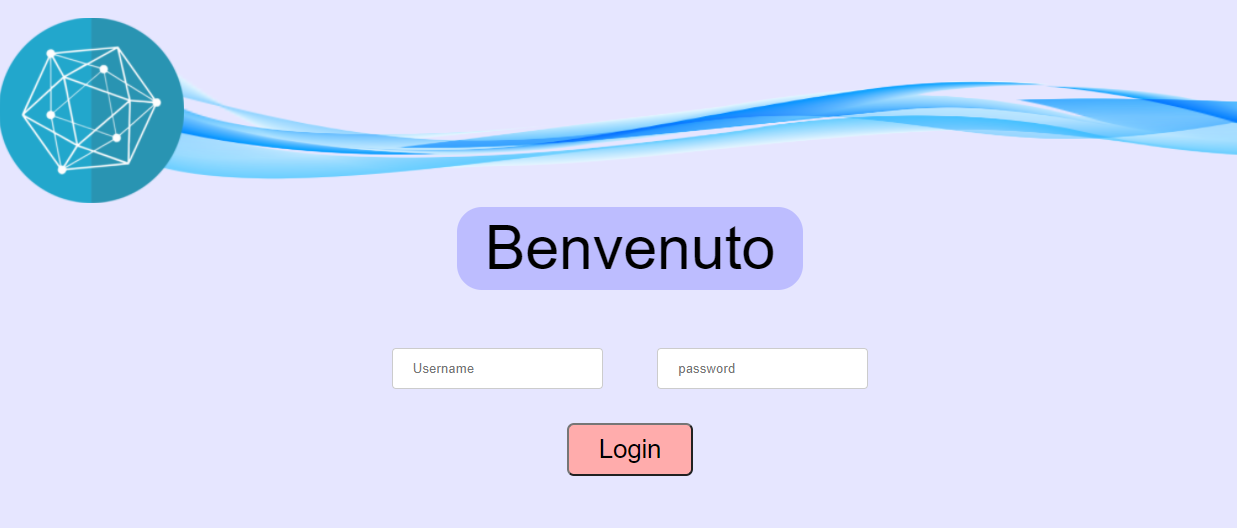
\includegraphics[width=\textwidth]{HomePage}
	\centering
	\caption{Schermata iniziale WebApp}
	\label{fig:besu-imported-produced}
\end{figure}

\subsection{Input}
Con Input dei dati viene indicato l'inserimento di essi in una specifica struttura di immagazzinamento dati. Per il progetto questo viene suddiviso in due azioni separate: input verso il DB, input verso la Blockchain.
\subsubsection{Inserimento in un DB}
Nel Database vanno ad essere salvati i dati di Log (~\ref{Schema-Progetto}), questi vengono inseriti dagli utenti salvati nel DB con Admin=False. Questi vengono inseriti in 2 instanti diversi tramite la SPA.
Nella prima schermata (\ref{fig:Init_Log}) si va ad inserire solo la città di partenze.
\begin{figure}[h]
	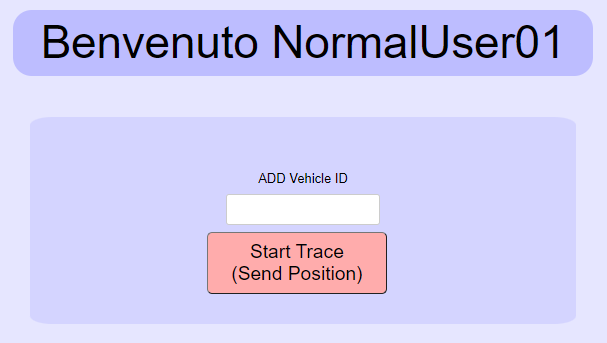
\includegraphics[width=\textwidth]{Init_Log}
	\centering
	\caption{Schermata iniziale Inserimento Log}
	\label{fig:Init_Log}
\end{figure}

Al termine si inserirà la città di destinazione e la distanza totale. Dati come lo Username e le date di inizio e di fine sono prese/calcolate autonomamente dal server.
\begin{figure}[h]
	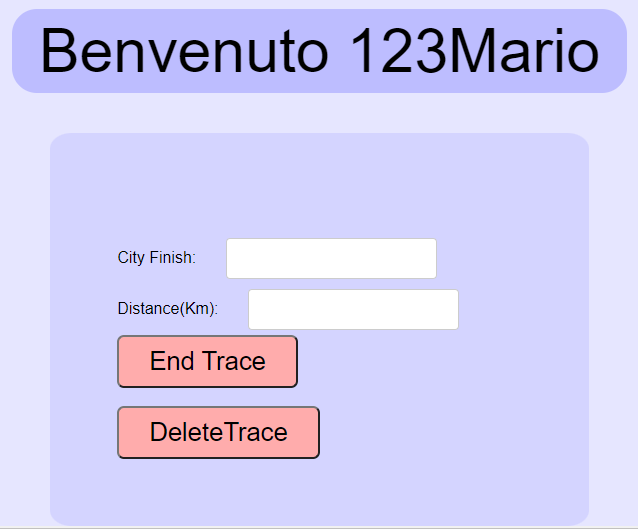
\includegraphics[width=\textwidth]{End_Log}
	\centering
	\caption{Schermata finale Inserimento Log}
	\label{fig:End_Log}
\end{figure}
Il DB viene connesso con il pacchetto \textit{mysql} ed ogni qualvolta un utente termina un Log viene salvato nel DB.
\begin{lstlisting}[language=JavaScript]
app.get('/SaveLog', (req,res) =>{
	var params = querystring.parse(url.parse(req.url).query);

	//Control Data
	if( params['cityFinish'].length==0 ||
		params['distance'].length==0) {res.json({result: false, ErrStr: "Campo/i Mancante"});return;}
	//Take id hash by DB +1
	LastID(req.session.busHex, (LastID, error) => {
		if(error) res.json({result: false, ErrStr: "Failed database connection " + error});
		else{
	  		ID_HASH= ++LastID;

	  		var dateFinish = DateNow();
	  		var connection = createConnectionDB();
		  	//save log in DB
		  	connection.query("INSERT INTO LOG (City_Start,City_Finish,UserName,Distance,DataStart,DataFinish,ID_HASH) VALUES(?,?,?,?,?,?,?)",
		  					[req.session.CityStartLog, params['cityFinish'], req.session.username, params['distance'], req.session.DateStartLog, dateFinish, ID_HASH ],
		  	function (error, results, fields) {
		  		if (error) res.json({result: false, ErrStr: "Failed database connection " + error});
		  		else res.json({result: true, ErrStr: ""});
			});
			connection.end();
	  	}
	});// LastID
});
\end{lstlisting}
La funzione \textit{LastID} interroga il Database così da ottenere per address specifico (si utilizza l'address salvato nella sessione \textit{req.session.busHex}) l'ultimo id di cui si è salvato l'hash, in questo modo si saprà quale id usare al prossimo log ( Ultimo id + 1).

\subsubsection{Inserimento nella Blockchain}
Il salvataggio dati sulla blockchain avviene periodicamente su un lasso di tempo specificato (24 ore per il progetto).
per il salvataggio si ha la necessità che un amministratore inserisca la private key.

Fino al momento che un amministratore non inserisca la Key, tutti gli account di utenti sotto quel determinato ente saranno impossibilitati dal server a salvare nuovi log. Allo scadere del lasso di tempo viene controllato dal DB chi (ente) ha inserito nuovi log che non sono stati salvati, viene di conseguenza impostato un blocco per gli utenti fino al momento del salvataggio (inserimento Private Key).

\begin{lstlisting}[language=JavaScript]
	setInterval(function(){
		// Set block to True for everyone that have add 'Log' in 24H
		var connection = createConnectionDB();
		connection.query("SELECT DISTINCT business_hex "
							+"FROM LOG as L JOIN terminaluser AS T ON (L.UserName= T.UserName) JOIN id_hash AS H ON(T.Business_Hex= H.Business)"
							+"WHERE NOT EXISTS(SELECT id_hash FROM id_hash WHERE id_hash= L.ID_HASH)",
		  	function (error, results, fields) {
		  		if (error) console.log(error);
		  		else results.forEach((row) => {if (BlockHex.indexOf(row.business_hex)===-1) BlockHex.push(row.business_hex);});
		});
		connection.end();
	}, oneDay);
\end{lstlisting}

\begin{figure}[h]
	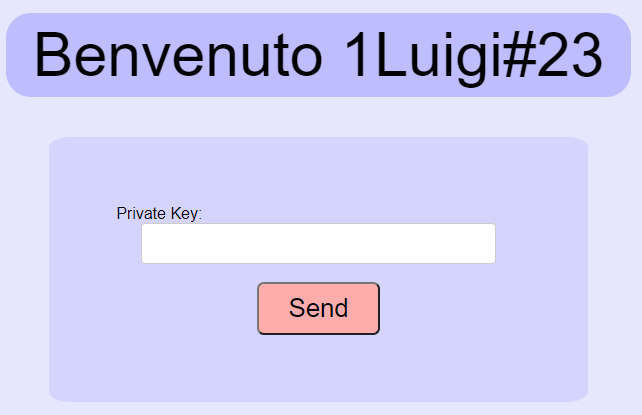
\includegraphics[width=\textwidth]{Input_Key}
	\centering
	\caption{Schermata Inserimento Private Key}
	\label{fig:Input_Key}
\end{figure}

\subsection{Output}
\subsubsection{Report di Controllo}
\subsubsection{Monitor Blockchain}

\subsection{Input}
\begin{thebibliography}{1}
\bibitem{} \url{https://besu.hyperledger.org/en/stable/Tutorials/Private-Network/Create-IBFT-Network/} come creare una rete blockchain prvata con BESU
\bibitem{} \url{https://web3js.readthedocs.io/en/v1.5.2/}
\end{thebibliography}
%capitolo 6
\chapter{Sviluppi futuri}
\section{Analisi costi}
\section{Immissione nella blockchain pubblica}
\section{Blockchain pubblica come certificazione}
\section{Svilupo full Blockchain}


%lista delle Immagini
\listoffigures

\end{document}
